\begin{center}
\section*{\month}
\end{center}

\def\day{\textit{May 20st Simon, 2021}}
\def\weekday{\textit{Thursday}}
\subsection*{\weekday, \day}

onCreateView():

After the onCreate() is called (in the Fragment), the Fragment's onCreateView() is called. You can assign your View variables and do any graphical initialisations. You are expected to return a View from this method, and this is the main UI view, but if your Fragment does not use any layouts or graphics, you can return null (happens by default if you don't override).

Noah and were looking for my bug. And the conclusion was that the proble is how the RecyclerView is invoket in the MainActivity. The other problem is i can't 
copie it from the programm I used to. So I will look out how you use onCreatView in the Fragment or in oure term I think it is AppCompatActivity but that is not a Fragment so 
I have to look up somethings. 

\def\day{\textit{May 24st Noah, 2021}}
\def\weekday{\textit{Monday}}
\subsection*{\weekday, \day}

I changed \texttt{popup.xml} to use the Material Design ``TextInputLayout'' instead of the default ``TextEdit''. This allows for much more styling usefule extra features. This lead to me restyling the newemailpopup.\\

Then I added input validation: For the Name and Password I only have to check that the string is not empty, but for the email I additionaly used a regex the see if the email is valid. It looks like this:\\

\begin{figure}[H]
\centering
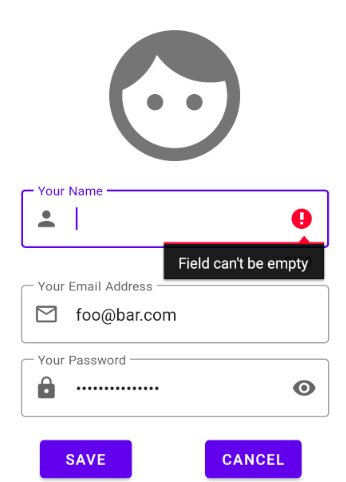
\includegraphics[height=.3\textheight]{media/newemail}
\end{figure}

When the Input is correct, a new windows will popup that I styled in \texttt{provider\_database\_checker.xml}. I named it that at first, because between the first popup and this it should check if the email domain is in the database of providers. Whatever, in this email you can customize the exact connection settings like port, imap/smtp server and SSL Encryption.\\

I also added two functions to ``MainActivity.java'', namely ``showSnackbar'' and ``showToast''. These are very useful for different debugging output purposes.
